\section{Results}
\label{Results}

\subsection{Spatial variability of water conditions and habitats}

There were significant differences between both islands (\textit{p}<0.05; Wilcoxon rank sum test) in some of the measured water variables (Table S4.1). In Floreana, nitrite and sulfate concentrations were significantly higher, while in Santa Cruz ammonium concentrations, temperature, pH and DO concentrations were significantly higher. Although not significant, nitrate, phosphate, total P and chlorophyll concentration were on average higher in Santa Cruz than in Floreana, while total N and EC were on average higher in Floreana. Although rocky habitats were targeted for the transects, sandy patches were often unavoidable and sand cover was significantly higher in Santa Cruz (the abiotic data is depicted visually in PCA plots (Figures S4.1, S4.2 and S4.3). PERMANOVA tests using all available water variables also highlighted significant differences in water quality between both islands (\textit{p}<0.05), and the lack of significant differences in distances to the centroids (PERMDISP tests) suggests that the significant PERMANOVA was due to true differences in multivariate water quality data rather than to differences in variability. However, when PERMANOVA was performed only on the selection of water parameters identified in section \ref{Fishassemblagestructure} as potential drivers of the structure of fish assemblages (temperature, ammonium, phosphate, nitrite and sulfate concentration), both PERMANOVA and PERMDISP yielded significant results, showing a higher multivariate dispersion among locations in Santa Cruz than in Floreana and potentially questioning a significant island effect on the abiotic environment. However, the CAP leave-one-out cross-validation misclassification error was exactly 0 \%, suggesting that both islands could still be perfectly distinguished from each other based on their water parameters. 

Similarly, PERMDISP tests indicated a significantly larger variability of the physical habitats among locations in Santa Cruz compared to Floreana. Here, PERMANOVA tests were only marginally significant (\textit{p}<0.1), suggesting that there were no clear differences in habitat classes between both islands, in addition to the difference in variability. This was supported by the high CAP leave-one-out cross-validation misclassification error (20 \%; note that a misclassification error of 50 \% is expected by chance alone). Between locations, no significant differences were found for both PERMDISP and PERMANOVA.

Coliforms and \textit{E. coli} were found more often in Santa Cruz than in Floreana (Table S4.2). In three out of three locations in Santa Cruz both coliforms and \textit{E. coli} were found, while in Floreana, the respective frequencies were three out of five and one out of five locations. 

\FloatBarrier

\subsection{Fish $\alpha$ and $\beta$ diversity}

The linear mixed models did not indicate any significant difference in point species richness between both islands (\textit{p}>0.05). Similarly, Wilcoxon rank sum tests did not indicate any significant difference in sample species richness. The total amount of species recorded in Santa Cruz and Floreana was 39 and 33, respectively (Figure S5.1). There was a significant effect of the factor Location in the linear mixed models for the locations, irrespective of the islands. Pairwise comparisons with Tukey correction of these models revealed significantly higher point species richness in location B9 compared to locations C1, B3 and B6; and in location C4 compared to location B3. 

$\beta$ diversity among locations was significantly larger in Santa Cruz than in Floreana (\textit{p}<0.05), indicating stronger variability in species composition in Santa Cruz (Figure S5.2). The distance-to-centroid for Santa Cruz was on average 31.8 \% (SE of 2.4 \%) while for Floreana it was only 17.5 \% (SE of 2.4 \%). Pairwise comparisons between locations, without correction for multiple comparisons, did only result in some marginally significant differences (\textit{p}<0.1) in $\beta$ diversity. However, it should be noted that the number of transects per location was limited to three, impeding strong statements on potential differences between locations due to limited statistical power. The range of distance-to-centroid values was quite large, from 3.82 \% to 27.63 \%, but more data is required to assess the $\beta$ diversity at this fine spatial scale (Table S5.4 and Figure S5.2).

There was only a limited amount of significant correlations between diversity measures and environmental variables. Nitrite concentration was negatively correlated with the sample species richness of locations in Floreana (\textit{r}=-0.96). In Santa Cruz, Total P concentration (\textit{r}=-0.94) and habitat class sediment deposition on rocks (\textit{r}=-0.91) were negatively correlated with point species richness, while EC was positively correlated (\textit{r}=0.94) with point species richness (Table S5.2). Although not all types of nutrient concentrations showed significant correlations with point species richness and sample species richness, correlations between nutrient concentrations and point species richness and sample species richness were always negative in Santa Cruz. In Floreana, on the other hand, there were both positive and negative non-significant correlations between nutrient concentrations and point species richness and sample species richness. In Floreana, $\beta$ diversity was positively correlated with nitrate (\textit{r}=0.91) (Table S5.3). In Santa Cruz, $\beta$ diversity was negatively correlated with DO (\textit{r}=-0.92) and sand cover (\textit{r}=-0.88 ). A positive, but not significant (\textit{p}=0.13), Pearson correlation (\textit{r}=0.52) was found between $\beta$ diversity and physical habitat variability (Table S5.4). 

\FloatBarrier

\subsection{Fish assemblage structure}
\label{Fishassemblagestructure}

PERMDISP tests on the full biological data set indicated significant heterogeneity of multivariate dispersion at the level of islands, locations and transects (\textit{p}<0.05), but not at the level of the Observers. Multivariate variability was significantly larger for Santa Cruz than for Floreana, as the average distance-to-centroid of Santa Cruz was 35.44 \% (SE=0.48 \%), while for Floreana it was only 27.30 \% (SE=0.49 \%). PERMANOVA models revealed significant effects at the level of islands and locations (\textit{p}<0.05). Within the island of Santa Cruz, more significant differences (\textit{p}<0.05) were found between locations (B10-B3; B10-B6; B10-B9; B3-B9; B6-B9) than between the locations of Floreana (C1-C4). The \textit{p}-values were not corrected since the permutation \textit{p}-values provide an asymptotically exact test of each individual null hypothesis of interest \citep{Anderson2008PERMANOVA+Methods}\footnote{Because an asymptotically exact test was performed using a large number of permutations, it is reasonable to assume that the p-values and family-wise error rate (chance of at least one type I error (incorrect rejection of null hypothesis)) are not underestimated. Hence, with 10 comparisons and a 5\% significance level it would be expected that 0.5 rejections are due to chance (i.e. family-wise error rate). Since there were 5 significant rejections of the null hypothesis it is unlikely that all of them were due to chance. The family-wise error rate hampers the exact identification of the real differences (as some of the differences might actually not be a difference), but does allow a relatively strong statement regarding the large number of significantly different locations within Santa Cruz, compared to within Floreana}. Because PERMDISP and PERMANOVA analyses both yielded significant results, there was not necessarily a significant difference in the structure of the fish assemblages in addition to the difference in variability. However, CAP discriminant misclassification errors were generally low, indicating that the locations and transects of both islands could be relatively well distinguished from each other. Hence, the structure of the fish assemblages differed between islands, locations and transects. Differences among locations and transects were clearer (i.e., had lower misclassification errors) at Santa Cruz than at Floreana (Tables S8.1, S8.2, S8.3 and S8.4). These results are clearly visualized in the PCO plot, where the fish assemblages of both islands were clearly separated (Fig. \ref{fig:PCO_Location_full}), and where there is much more overlap among locations at Floreana than at Santa Cruz (Figures S7.1 and S7.2). In addition to the factors Island (Table S6.1: 57.09 \%) and Location (12.47 \%), the factor Transect also explained a substantial part of the variation (12.74 \%), whereas the factor Observer alone explained a negligible fraction of the data variation (0.27 \%). The interaction of Observer with the factors Island (0.06 \%), Location (2.97 \%), and Transect (4.39 \%) still never explained more than 7.5 \% of the observed variation. In Santa Cruz, variability explained by the locations (38.05 \%) was larger than the variability explained by the transects (28.72 \%), while the opposite was true for Floreana (i.e. locations and transects explained 16.62 \% and 17.60 \% of the variation, respectively). 

In both Santa Cruz and Floreana, Endemic, Peruvian, Indo-Pacific, Panamic and widespread species were observed (Table S5.1). Using the correlations of the biological data with the first PCO axis, the differences between islands could be partly attributed to some typical species. For Santa Cruz, these included the Bullseye puffer fish (\textit{Sphoeroides annulatus}; \textit{r}=-0.62), Yellowtail damselfish (\textit{Microspathodon bairdii}; \textit{r}=-0.83) and Pacific spotfin mojarra (\textit{Eucinostomus dowii}; \textit{r}=-0.64), while for Floreana they comprised the Bravo clinid (\textit{Gobioclinus dendriticus}; \textit{r}=0.56), Galapagos ringtail damselfish (\textit{Stegastes beebei}; \textit{r}=0.83) and Chameleon wrasse (\textit{Halichoeres dispilus}; \textit{r}=0.87). In Santa Cruz, the abundances of the Yellowtail damselfish and Pacific spotfin mojarra were positively correlated with DO and pH, while the abundances of the Bullseye puffer fish were positively correlated with phosphate and negatively correlated with EC. In Floreana, the abundance of the Galapagos ringtail damselfish was positively correlated with nitrite, while that of the Bravo clinid was negatively correlated with the percentage of bare rock and that of the Chameleon wrasse was positively correlated with phosphate. 

\begin{figure}[h!]
  \centering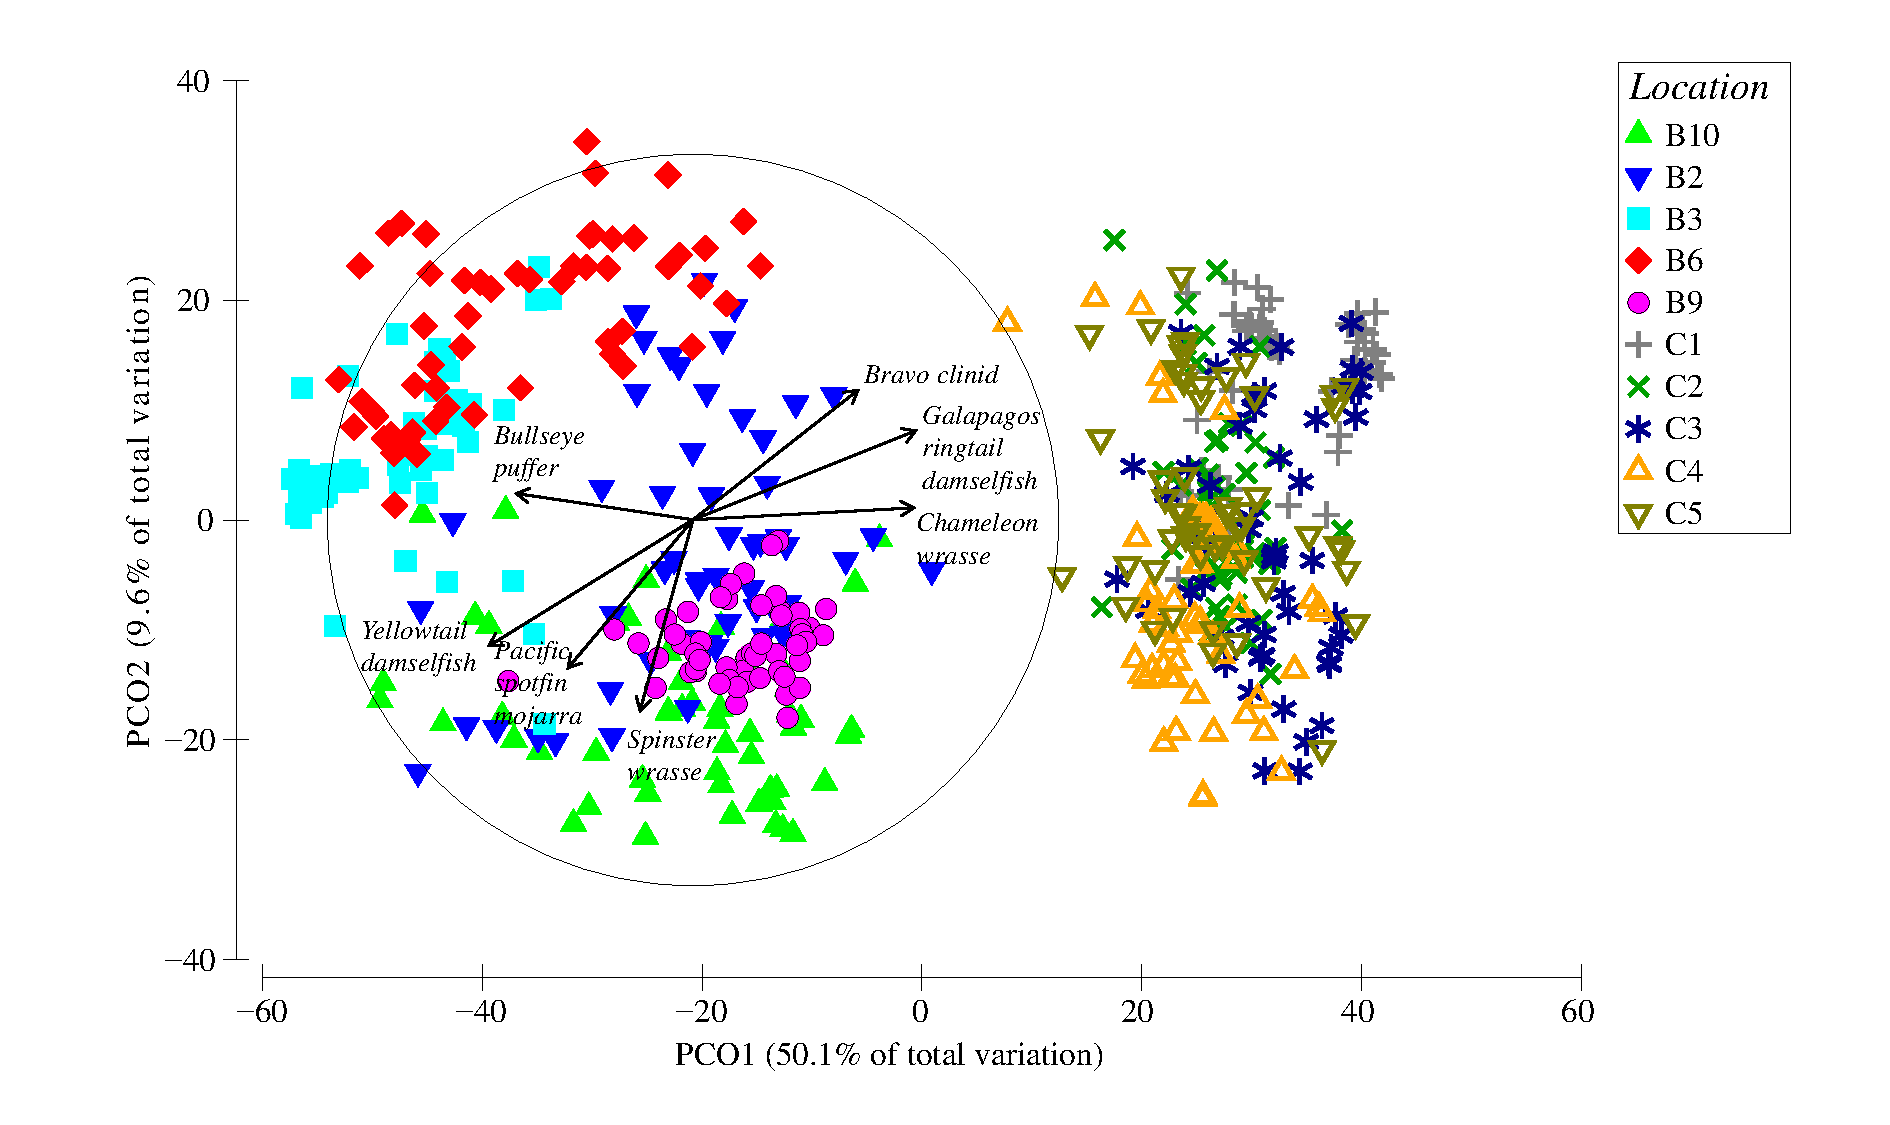
\includegraphics[scale=0.42]{PCO_with_species}
  \caption{PCO based on Bray-Curtis resemblance matrix with distinction of the different locations in Santa Cruz (locations B) and Floreana (locations C). The fish species with a Pearson correlation of more than 0.4 with the ordination axes are represented as vectors.} 
  \label{fig:PCO_Location_full}
\end{figure}

\FloatBarrier

The squared canonical correlations of PC1 with CAP1 indicate how well differences in the structure of fish assemblages can be explained by the water conditions, physical habitats and geographical distance. Compiling data of both islands, these correlations (n=30) were quite high: 0.85, 0.66 and 0.90, respectively (Table \ref{can_correl_CAP_Transectlevel_Median}). At the level of individual islands, the squared correlations were 0.75, 0.76 and 0.36 for Santa Cruz (n=15), while for Floreana (n=15), they were much lower: 0.03, 0.28 and 0.16, respectively. 

When focusing on water conditions, the most parsimonious model that best explained fish community variation for both islands contained five variables: Temperature, ammonium, phosphate, nitrite and sulfate (q=5). When focusing on the habitats, three variables were retained in the most parsimonious model: Cover of vegetated rock, bare rock and rock with sediment deposition (q=3). When focusing on the geographical distance, Y and X$^{3}$ were retained in the most parsimonious model (q=2). For Santa Cruz, total P and temperature (q=2), cover of rock with sediment deposition (q=1) and Y$^{3}$, X and Y (q=3) were retained. For Floreana, nitrite (q=1), cover sand and bare rock (q=2) and X$^{3}$ (q=1) were retained (Table S9.1).  

For the full data set, water conditions explained the largest share of the variation, followed by the geographical distance and physical habitats (marginal tests in Table \ref{DISTLMseries_Transectlevel_Median}). The sequential conditional tests indicated that the most parsimonious model contained only geographical distance. If geographical distance was not included, the most parsimonious model only comprised water conditions. Changing the number of variables per subset of each series (i.e. geographical distance, water conditions and physical habitats) did not change the order of importance of the series, but did affect the number of series to be included in the parsimonious model (Table S9.3).

Within each island, geographical distance was not included in the most parsimonious models (Table \ref{DISTLMseries_Transectlevel_Median}). Indeed, the sequential conditional tests for Floreana only retained physical habitats to explain the structure of the fish assemblages, while for Santa Cruz only water conditions were retained in the most parsimonious model. However, for Santa Cruz, the AICc of the model using solely geographical distance was only slightly higher ($\Delta$AICc$\textless$2). In addition, care should be taken when comparing these results, because the number of variables included in the subsets had an effect on the order and nature of the series retained in the parsimonious model of Santa Cruz (Table S9.2). If one instead of two variables per series were included, both physical habitat and geographical distance were added to the parsimonious model, but water conditions were left out (Table S9.2). For Floreana there was no effect of the number of variables on the order or nature of included series. To visualize the outcomes of these models ordinations of their fitted values are represented in Figs S9.1, S9.3, S9.4, S9.6, and S9.7. As the main patterns of the unconstrained PCO ordination plots (Figs S9.2, S9.5, and S9.8) and constrained dbRDA plots are relatively similar\footnote{Comparison of original values and fitted values respectively \citep{Anderson2008PERMANOVA+Methods}}, the models appear adequate to find and explain the most important patterns in the data. 

When no prior clustering of predictors in series (water conditions, physical habitats or geographical coordinates) was done, a parsimonious model for the full data set contained the predictors Y, cover of rock with sediment deposition, temperature, ammonium concentration and cover of vegetated rock (Table \ref{DISTLMallvariablesoutsideseries_Transectlevel_median}). For Santa Cruz, a two-variable model containing cover of rock with sediment deposition and temperature was considered best, while for Floreana a two variable model containing cover of sand and bare rock was optimal.

\renewcommand{\arraystretch}{1.25}
\begin{table}
\centering
\scriptsize
\caption{Squared canonical correlations of the first PCA axis (PC1) with the first CAP axis (CAP1) for the different series of variables: Water parameters (Water), physical habitats (Habitat) and geographical distances (XY) for both islands together (n=30) and separately (n=15).}
\label{can_correl_CAP_Transectlevel_Median}
\begin{tabular}{@{}l|P{2cm}P{2cm}P{2cm}@{}}
\toprule
                                                                      Variable series  & Both islands & Santa Cruz & Floreana  \\ 
\midrule
~Water       & 0.85         & 0.75       & 0.03       \\ 
~Habitat & 0.66         & 0.76       & 0.28       \\
~XY       & 0.90         & 0.36       & 0.16       \\ 
\bottomrule
\end{tabular}
\end{table}
\renewcommand{\arraystretch}{1}

\renewcommand{\arraystretch}{1.5}
\begin{table}
\centering
\scriptsize
\caption{Results of DISTLM analyses using series of predictors (water parameters (Water), physical habitats (Habitat) and geographical distances (XY)). The optimal number of predictors per series was determined using the AICc. For each marginal test also the AICc weights (w\textsubscript{AICc}) were determined. Models were constructed for both islands together (n=30) and separately (n=15).}
\label{DISTLMseries_Transectlevel_Median}
\resizebox{0.7\textwidth}{!}{
\begin{tabular}{@{}l|l|P{12mm}P{1cm}P{1cm}P{12mm}P{12mm}|P{12mm}P{1cm}P{12mm}@{}}
\toprule
\multirow{2}{*}{}                                                        & \multirow{2}{*}{Variable series} & \multicolumn{5}{c|}{Marginal tests}  & \multicolumn{3}{c}{Sequential tests}  \\ 
%\cline{3-9}
                                                                         &                               & pseudo-F & p-value     & R$^{2}$  & AICc & w\textsubscript{AICc}  & pseudo-F & p-value     & cum. R$^{2}$        \\ 
\midrule
\multirow{3}{*}{\begin{tabular}[c]{@{}l@{}}Both \\islands \end{tabular}} & XY (q=2)                      & 21.43    & 0.001 & 0.61     & 202.11 & 0.73 & 21.43    & 0.001 & 0.61                \\ 
                                                                         & Water (q=5)                   & 10.71    & 0.001 & 0.69     & 204.18 & 0.26     & /        & /     & /                   \\ 
                                                                         & Habitat (q=3)                 & 9.03     & 0.001 & 0.51     & 211.89 & 0.01    & /        & /     & /                   \\ 
\hline
\multirow{3}{*}{\begin{tabular}[c]{@{}l@{}}Santa \\Cruz \end{tabular}}   & Water (q=2)                   & 5.52     & 0.001 & 0.48     & 103.17 & 0.48 & 5.52     & 0.001 & 0.48                \\
& XY (q=3)                      & 4.95     & 0.001 & 0.58     & 103.96 & 0.32     & /        & /     & /                   \\ 
                                                                         & Habitat (q=1)                 & 4.91     & 0.001 & 0.27     & 104.97 & 0.20     & /        & /     & /                   \\ 
                                                                         
\hline
\multirow{3}{*}{Floreana}                                                & Habitat (q=2)                 & 4.00     & 0.001 & 0.40     & 94.46 & 0.66 & 4.00     & 0.001 & 0.40                \\ 
& XY (q=1)                      & 1.74     & 0.144 & 0.12     & 97.06 & 0.18     & /        & /     & /                   \\
                                                                         & Water (q=1)                   & 1.56     & 0.187 & 0.11     & 97.24 & 0.16     & /        & /     & /                   \\ 
                                                                         
\bottomrule
\end{tabular}
}
\end{table}
\renewcommand{\arraystretch}{1}

\renewcommand{\arraystretch}{1.25}
\begin{table}
\centering
\scriptsize
\caption{Results of DISTLM analyses using all predictors, without grouping them in different series of variables. Predictors were selected using AICc. For both islands together (n=30) and separately (n=15).}
\label{DISTLMallvariablesoutsideseries_Transectlevel_median}
\resizebox{0.7\textwidth}{!}{
\begin{tabular}{@{}l|l|P{12mm}P{1cm}P{1cm}|P{12mm}P{12mm}P{10mm}P{12mm}@{}}
\toprule
\multirow{2}{*}{}                                                        & \multirow{2}{*}{Variable}                                                                & \multicolumn{3}{c|}{Marginal tests} & \multicolumn{4}{c}{Sequential tests}  \\ 
                                                                         &                                                                                          & pseudo-F & p-value     & R$^{2}$          & AICc & pseudo-F & p-value     & cum. R$^{2}$        \\ 
\midrule
\multirow{5}{*}{\begin{tabular}[c]{@{}l@{}}Both \\islands \end{tabular}} & Y (latitude)                                                                                        & 32.81    & 0.001 & 0.54    &    204.89     & 32.81    & 0.001 & 0.54                \\ 
                                                                         & \begin{tabular}[c]{@{}l@{}}Rock with\\sediment deposition \end{tabular} & 9.08     & 0.001 & 0.24      &   201.96    & 5.33     & 0.001 & 0.62                \\ 
                                                                         & Temperature                                                                              & 19.37    & 0.001 & 0.41      &   200.09    & 4.25     & 0.001 & 0.67                \\ 
                                                                         & Ammonium                                                                                 & 17.45    & 0.001 & 0.38     &   199.26     & 3.31     & 0.004 & 0.71                \\ 
                                                                         & Vegetated rock                                                                           & 9.95     & 0.001 & 0.26     &    199.18    & 2.73     & 0.012 & 0.74                \\ 
\hline
\multirow{2}{*}{\begin{tabular}[c]{@{}l@{}}Santa \\Cruz \end{tabular}}   & \begin{tabular}[c]{@{}l@{}}Rock with\\sediment deposition \end{tabular} & 4.91     & 0.001 & 0.27      &   104.97    & 4.91     & 0.002 & 0.27                \\ 
                                                                         & Temperature                                                                              & 4.00     & 0.003 & 0.24      &   102.66    & 5.30     & 0.002 & 0.50                \\ 
\hline
\multirow{2}{*}{Floreana}                                                & Sand                                                                                     & 3.94     & 0.003 & 0.23     &    94.97    & 3.94     & 0.004 & 0.23                \\ 
                                                                         & Bare rock                                                                                & 3.31     & 0.011 & 0.20     &    94.47    & 3.34     & 0.023 & 0.40                \\
\bottomrule
\end{tabular}
}
\end{table}
\renewcommand{\arraystretch}{1}

\FloatBarrier